\subsection{Setup}
In the experiments we downcase all  text  and use the BERT models ``bert-base-uncased" and ``bert-large-uncased". We implemented all experiments using the transformers library \citep{wolf2019huggingfaces}.

To compute the rotation matrices by DensRay, we need the
labels of a gendered word list and a corpus. For the word
list, we get 23 masculine words and 23 feminine words from
the ``family''
category,\footnote{http://download.tensorflow.org/data/questions-words.txt}
of the Google analogy test set \citep{mikolov2013efficient}
and label them as 1 and -1. As the input corpus, we collect
text data from Wikipedia that contains 5,000 (resp.\ 10,000)
occurrences of words in the gendered list for the BERT base
(resp.\ large) model. We carefully balance the occurrences such that the number of male and female samples are equal. We set  $\alpha_{\neq}=\alpha_{=}=0.5$, as we have balanced the training samples from the corpus.

We compare with the post-processing method proposed by
\citet{mu2018all} to eliminate gender bias as
introduced by \citet{karve2019conceptor}. \enote{hs}{do you
  mean: ``as
  adapted to contextualized embeddings by \citet{karve2019conceptor}''?}

\subsection{Results on OCCTMP}
\tabref{t:templates1} gives results for OCCTMP. Two OCCTMP
examples are given in \tabref{t:templates2}. It shows that
DensRay can mitigate the gender bias in BERT: the average
difference between predicting he/she drops to around two
third (e.g., for bert-base from 0.47 to 0.11).

\enote{hs}{there is a summarizing sentenc emissing jhere:
  performance of hard debiaisig and densray are comparable}

\begin{table}[ht]
\centering
\footnotesize
\begin{tabular}{lcccc}
\hline
model & prob(he) & prob(she) & diff & var\\
\hline
bert-base & 0.66 & 0.19 & 0.47 &0.16\\
bert-base-Mu & 0.35 & 0.42 & -0.07  &0.03\\
bert-base-densray & 0.48 & 0.37 & {0.11} &0.02\\
\hline
bert-large  & 0.63 & 0.19 & 0.44  &0.13\\
bert-large-Mu & 0.40 & 0.23 & 0.17  &0.02\\
bert-large-densray  & 0.47 & 0.31 & {0.16} &0.02 \\
\hline
\end{tabular}
\caption{\tablabel{t:templates1} BERT debiasing results on
  OCCTMP. \textit{bert-base} and \textit{bert-large} are the
  original models without debiasing. \textit{prob(he)} is
  the average probability  predicted for \textit{he} as
  the [MASK] in OCCTMP. \textit{var} is the variance of the
  differences between the probabilities of  predicted
  for \textit{he} and \textit{she}. \enote{pd}{why
    don't we compare with conceptor anymore?}}
\end{table}
\begin{table}[ht]
\centering
\footnotesize
\begin{tabular}{llcc}
\hline
sentence & model & prob(he) & prob(she)\\
\hline
[MASK] is a & 
\scriptsize bert-base 
& 0.72 & 0.19\\
adjunct professor. & 
\scriptsize bert-base-densray 
& 0.44 & 0.47\\
&\scriptsize bert-large
& 0.72 & 0.22\\
&\scriptsize bert-large-densray& 0.40 & 0.53\\
\hline
[MASK] is a 
&\scriptsize bert-base 
& 0.63 & 0.23\\
administrator.  
&\scriptsize bert-base-densray 
& 0.50 & 0.38\\
&\scriptsize bert-large & 0.65 & 0.23\\
&\scriptsize bert-large-densray & 0.45 & 0.37\\
\hline
\end{tabular}
\caption{\tablabel{t:templates2}
OCCTMP examples with prediction probabilities.}
\end{table}

\enote{hs}{since ``a adjunct'' and ``a administrator'' are
  not correct english, can you please find examples that are
  correct english?}

\subsection{Results on WEAT}
In WEAT we measure the effect size $d$-value and the
onesided $p$-value of the permutation test.  A $d$-value
closer to zero indicates less gender bias.  We also prefer a
high $p$-value (at least 0.05) to not reject the null
hypothesis, i.e., we do not reject that there is no gender
bias. We use \citet{karve2019conceptor}'s WEAT word list
setup.
\tabref{t:weat1} shows
results on WEAT.


\enote{hs}{there is a summarizing sentenc emissing jhere:
  performance of hard debiaisig and densray are comparable
  (although results are somewhat random as we have discussed before)}


\begin{table}[ht]
\centering
\scriptsize
\begin{tabular}{clcccc}
\hline
&&\multicolumn{2}{c}{WEAT}&\multicolumn{2}{c}{SEAT}\\
\hline
category & model & d & p& d & p\\
\hline
C6 & bert-base & 0.66 & 0.08 &0.11&0.25\\
& bert-base-Mu & 0.15 & 0.38&0.48&0.10\\
&bert-base-densray & 0.62 & 0.12&-0.11&0.75\\
%& bert-large & 1.57 & $0.00^{*}$ \\
%&bert-large-Mu & 0.80 & 0.06 \\
%& bert-large-densray & 0.76 & 0.07\\
\hline
C7 & bert-base & 0.60 & 0.11 &0.72&0.01\\
& bert-base-densray & -0.07 & 0.56&-0.09&0.72\\
& bert-base-densray & 0.09 & 0.45&-0.11&0.26\\
%& bert-large & -0.40 & 0.75 \\
%& bert-large-Mu & -0.51 & 0.83\\
%& bert-large-densray & -0.06 & 0.45\\
\hline
C8& bert-base & 0.78 & 0.08 &1.00&0.01\\
& bert-base-Mu & -0.29 & 0.68&0.36&0.03\\
& bert-base-densray & 0.03 & 0.47&0.75&0.01\\
%& bert-large & -0.60 & 0.87  \\
%& bert-large-Mu & 0.78 & 0.06\\
%& bert-large-densray & 0.20 & 0.33\\

\hline
\end{tabular}
\caption{\tablabel{t:weat1}
BERT debiasing results on WEAT. * shows significant gender bias.}
\end{table}

\enote{hs}{
``* shows significant gender bias'': i don't see any stars}

\subsection{Impact on Model Performance}
It is crucial that debiasing methods do not harm downstream
performance of BERT models. Thus we test the perplexity of
language modeling on Wikitext-2
\citep{merity2016pointer}, a subset of Wikipedia with 2
million words. We also test on GLUE
\citep{wang2018glue}. For all the tests we follow the same
setup as
\citet{wolf2019huggingfaces}.\footnote{https://huggingface.co/transformers/} \tabref{t:glue1}
shows that DensRay debiasing gets comparable results with
the original models on Wikitext-2 and GLUE tasks.
\begin{table*}[ht]
\centering
\footnotesize
\begin{tabular}{lcccccccccc}
\hline
model & Wikitext-2&CoLA &SST-2&MRPC&STS-B&RTE&WNLI\\
\hline
bert-base &3.77&49.15&92.09&85.86&82.66&62.82&52.11\\
bert-base-mu &3.95&45.53&91.74&82.48&82.60&63.54&56.34\\
bert-base-densray &3.81&48.04&91.74&84.89&82.43&63.90&53.52\\
\hline
bert-large &3.29& 47.93&94.90&89.30&87.60&70.10&65.10\\
bert-large-Mu &3.85& 47.45&93.95&85.01&82.33&67.12&63.02\\
bert-large-densray &3.35& 48.91&94.02&88.84&85.63&67.78&64.48\\
\hline
\end{tabular}
\caption{\tablabel{t:glue1}
Language modelling perplexity and GLUE tasks
performance. \enote{pd}{it seems on bert-large densray is
  always better than Mu? Can't we make the argument that
  DensRay affects performance less?}\enote{hs}{great idea!}}
\end{table*}

\subsection{Discussions}
\subsubsection{Compare DensRay and Hard Debiasing}
\seclabel{artexample}
Here we compare the difference between DensRay and hard debiasing by \citep{mu2018all}. \figref{fig:example} shows artifically created two dimensional embeddings. The black lines show the gender directions identified by hard debiasing and DensRay. Hard debiasing does not use the labels of the male-female word pairs. Instead it relies upon the assumption that the first principal component of the considered vectors is a meaningful gender direction. This can fail in some cases. 

\enote{hs}{since this is a crucial point of the paper, we
  need a strong summary sentence here}


\begin{figure}[h]
	\centering
	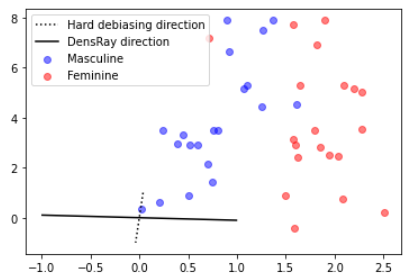
\includegraphics[width=0.9\linewidth]{example.png}
	\caption{Gender direction on gendered words. \enote{pd}{We should use the PCA with normalized data to make a fair comparison. Is this the case here?}}
	\figlabel{fig:example}
\end{figure}
\subsubsection{Debiasing on Attention Heads}
We now apply DensRay to the attention heads in BERT to
debias on OCCTMP, The heatmap \figref{fig:heads} shows that
the debiasing effect of one single attention head is not
obvious, with diff scores all in [0.4,0.5]. Due to the
lack of dimensions and the distribution of gender features
in the attention heads, we chose to apply DensRay on layers
as debiasing method.  We conclude that there is no single
attention head which is responsible for processing gender
information.
\begin{figure}[h]
	\centering
	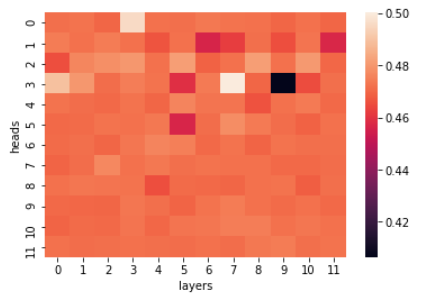
\includegraphics[width=0.9\linewidth]{heatmap_heads}
	\caption{DensRay debiasing on each single attention head in BERT base, measured by \text{diff} on OCCTMP.}
	\figlabel{fig:heads}
\end{figure}


\subsubsection{Number of Training Samples}
In the experiments, we collected training samples for
DensRay by considering occurrences of the same word in the
corpus across different sentences. We collected equally many
masculine and feminine words. Now we analyze the impact of
these processes.  DensRay is essentially a supervised
learning method. In the case of insufficient labels, it is
difficult for supervised learning to extract useful
features. Treating different occurrences as different words
greatly enriches training samples. As shown in
\figref{curve}, the debiasing results improve with an
increased number of training samples.

Similar to other projection-based debiasing methods
\citep{bolukbasi2016man,zhao2019gender,dev2019attenuating,
  karve2019conceptor}, the premise of DensRay debiasing is
that the bias direction should be correct. If the sample is
unbalanced, the bias direction computed by DensRay will be
biased towards either the male or the female, resulting in
deleting the gender subspace during debiasing and reversing
the gender bias. For example, if there are more masculine words in
unbalanced text data, then the embeddings will be biased
towards female after debiasing. The figure also shows that
a balanced training sample improves the debiasing
performance.
\enote{hs}{i don't understand the last point: does the
  figure also show experimental results for balanced vs
  unbalanced training sets?}
\begin{figure}[ht]
    \centering
    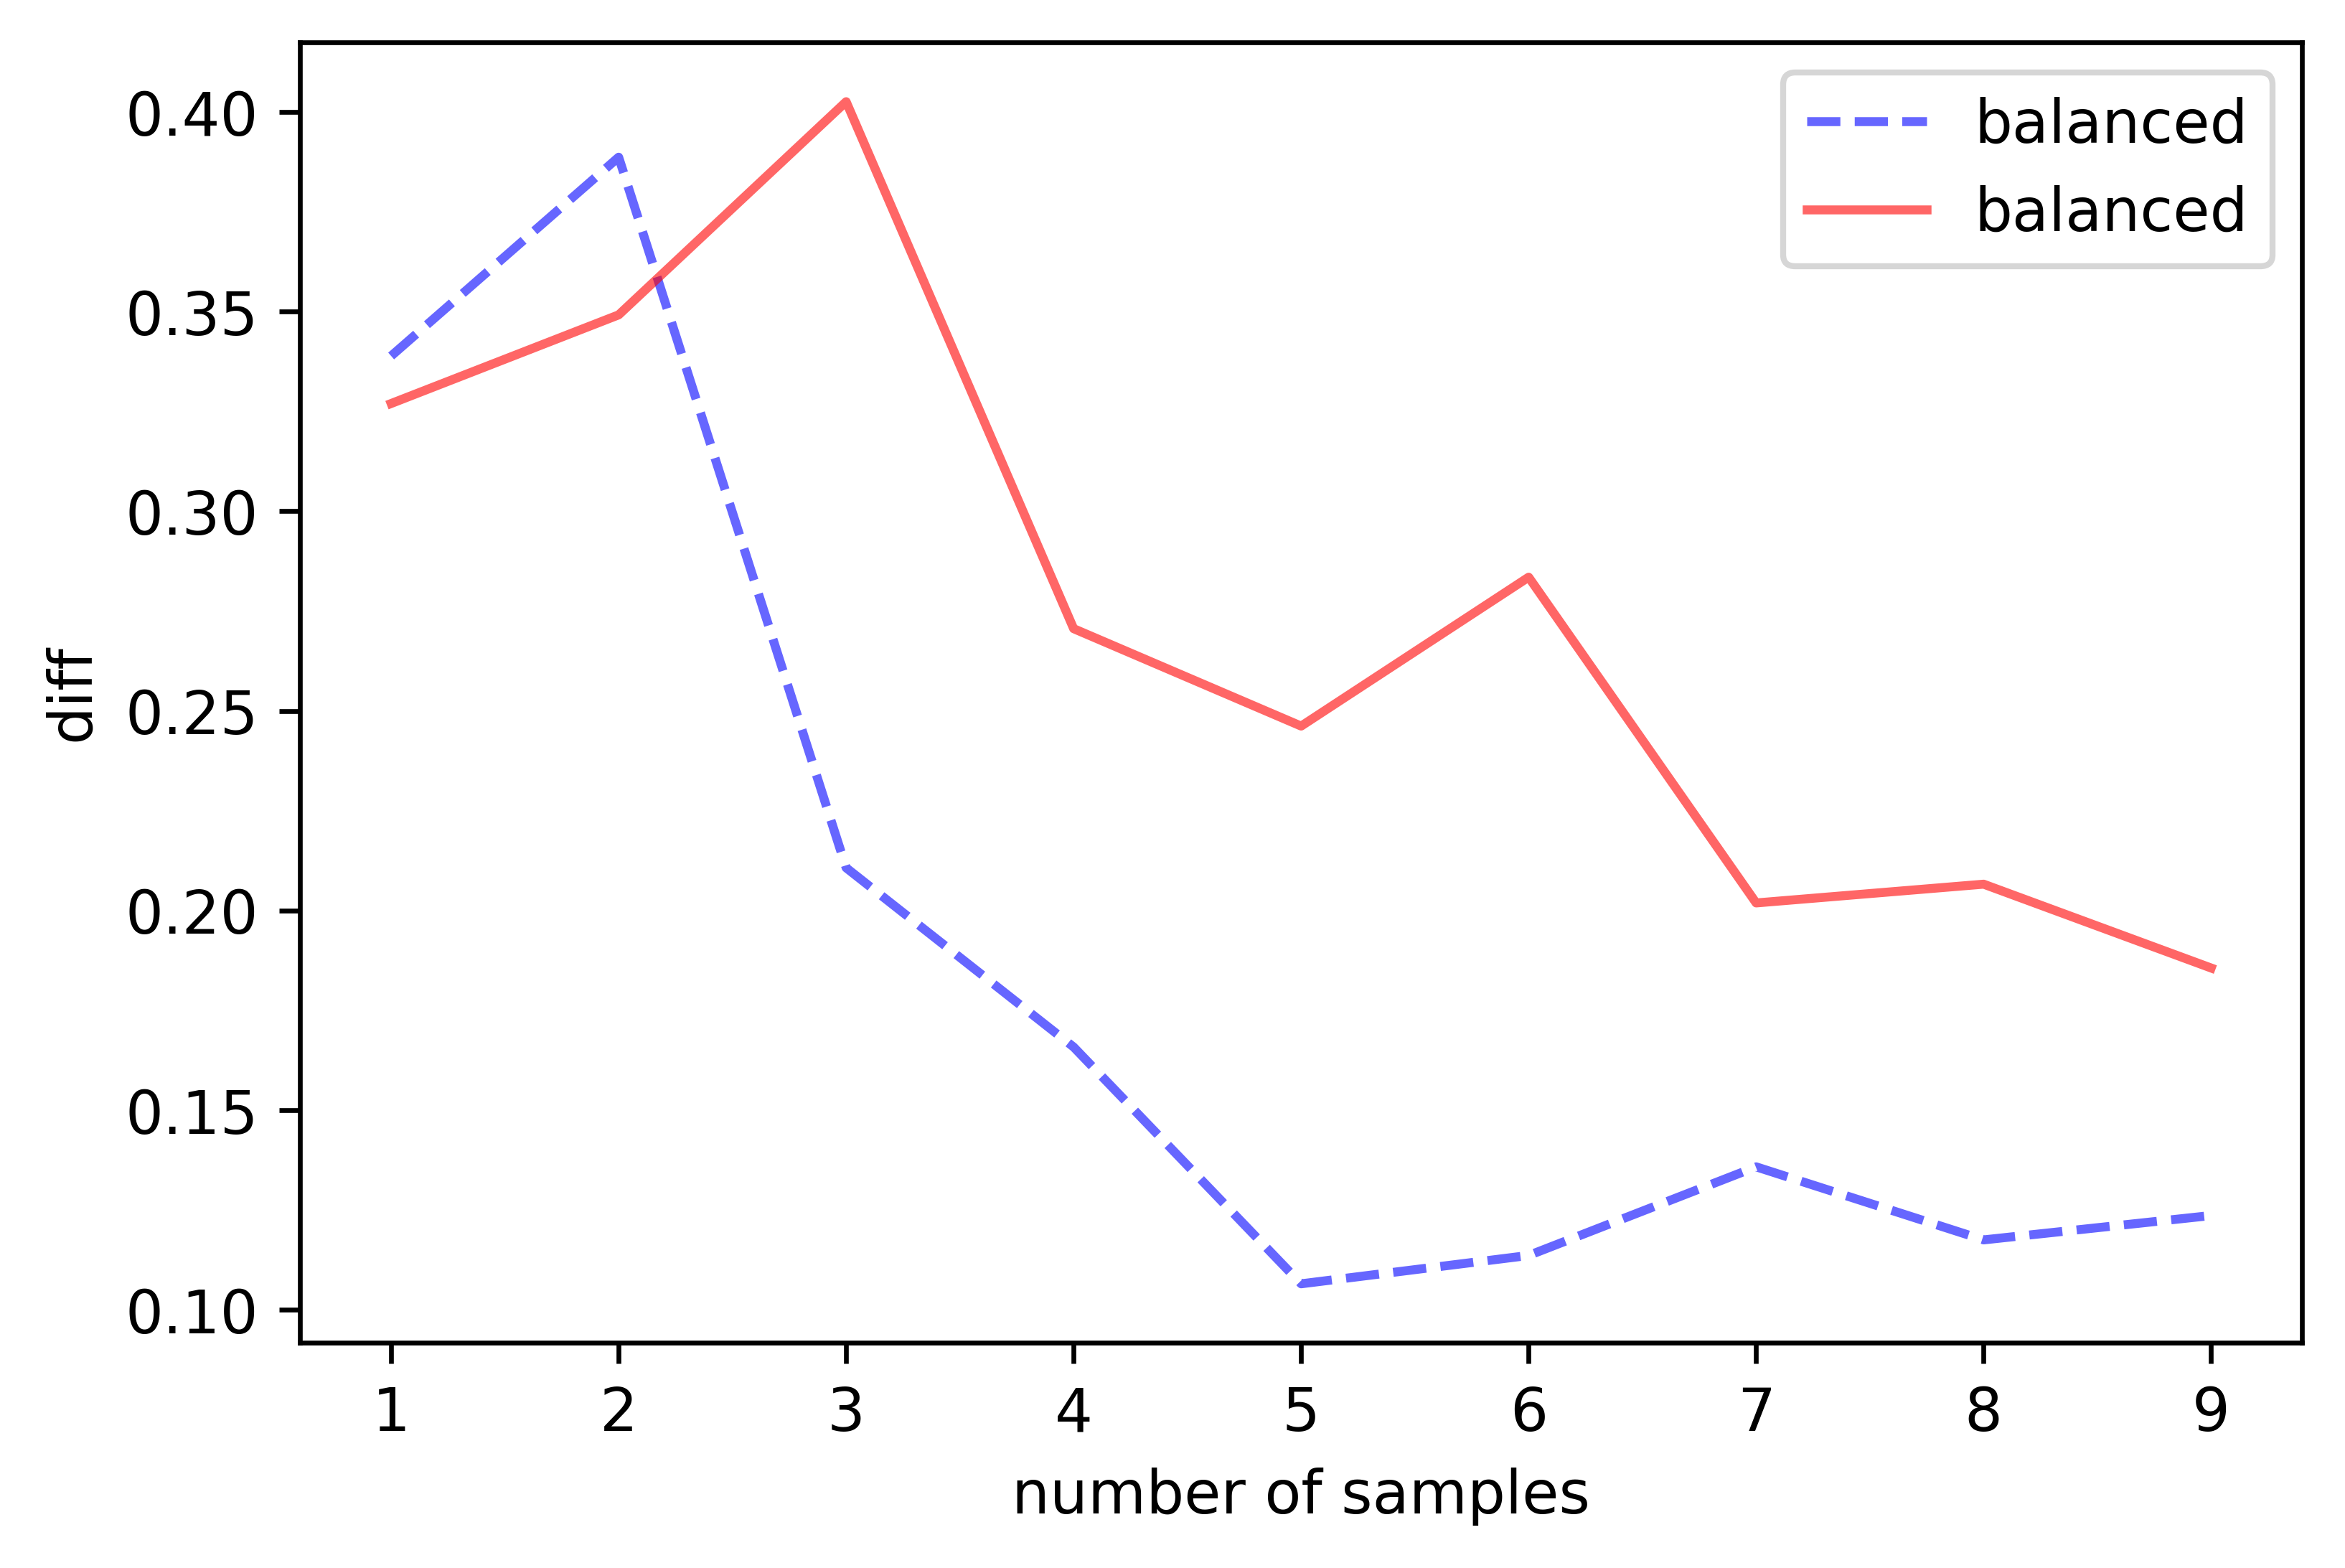
\includegraphics[width=6cm,height=3cm]{samples}
    \caption{DensRay debiasing results on OCCTMP with different number of samples.}
    \figlabel{curve}
\end{figure}

\subsubsection{Balancing Gender Bias}
\enote{pd}{I think this section can be moved to the supplementary material}
\enote{pd}{are we still targeting a short paper? or a long paper?}
In this experiment, we used the method of removing the first dimension (replacing its value by $0$) of the gender interpreteble subspace to remove gender bias. Here we explore some other ways.

We explored three other ways to remove bias: 1) replace the first dimension of the gender interpreteble subspace with the mean value of the first dimension of the training samples. 2) standardize the first dimension. 3) replace the first dimension with a small random variable sampled from Gaussian distribution. All of them did not perform well. We further checked the mean and found that the mean of the different layers is not stable around 0, which is a problem worthy for further exploring. We also tried to delete more dimensions. However removing more dimensions does not improve the debiasing results significantly, while harming the model performance significantly.


\subsubsection{Debiasing across different layers}
So far we have applied DensRay to all BERT layers simultaneously.
  \figref{fig:layersbase}  illustrates the effect of
 debiasing a single  layer on our templates and the three
 WEAT categories. We see that the debiasing effect
is stronger in
layers 7--10  than in the other layers in BERT base.
\begin{figure}[ht]
	\centering
	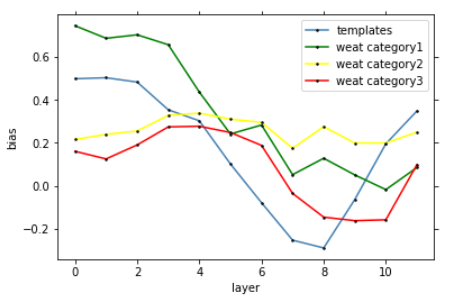
\includegraphics[width=0.9\linewidth]{layers_base}
	\caption{Debiasing on each single layer on BERT base. Bias is measured by \text{diff} on the templates and $d$-value on WEAT categories.}
	\figlabel{fig:layersbase}
\end{figure}

